\chapter{Variedades y Mapas}\label{Capítulo: Variedades y Mapas}
\section{Variedades Topológicas}\label{Sección: Variedades Topologicas}
Nuestro objeto de estudio fundamental serán las \it{variedades}, estos son espacios topológicos que localmente se asemejan a espacios euclidianos. En particular nos interesan las variedades que podamos dotar de una estructura suave, esto es, las variedades en las que podemos darle un significado a la derivada.

\begin{definition}[Variedad Topológica]\label{Definición: Variedad Topologica}
	Sea $M$ un espacio topológico, diremos que $M$ es una \it{variedad topológica $n$-dimensional} si:
	\begin{enumerate}
		\item $M$ es un \it{espacio de Hausdorff}; esto es, para cualesquiera par de puntos distintos $x_1,x_2$ de $M$ existen vecindades $U_1$ y $U_2$ de $x_1$ y $x_2$ respectivamente, que son disjuntas.
		\item $M$ es \it{segundo numerable}; esto es, la topología de $M$ tiene una base numerable.
		\item $M$ es \it{localmente Euclidiano} de dimensión $n$; esto es, para cada punto $x$ de $M$ existe una vecindad abierta $U \subset M$ que contiene a $x$ y una función $\phi: U \to \R^n$ continua y con inversa continua, i.e., un \it{homeomorfismo}.
	\end{enumerate}
\end{definition}

Para abreviar escribiremos \enquote{Sea $M^n$ una variedad topológica},  en lugar de escribir \enquote{Sea $M$ una variedad topológica $n$-dimensional}. Ocasionalmente, cuando no sea relevante, omitiremos escribir la dimensión de la variedad.

\begin{figure}[h]
	\begin{center}
		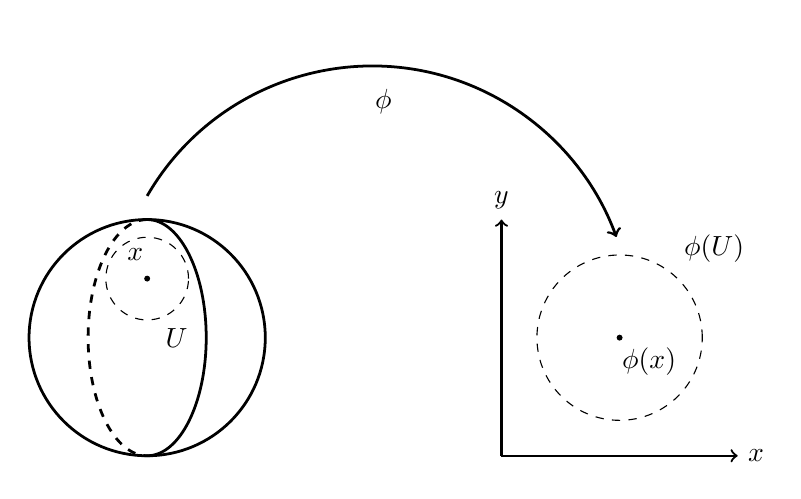
\begin{tikzpicture}[scale=1.5]
  \draw[line width=1] (-3,2) arc (90:-90:0.5 and 1);
  \draw[line width=1, dashed] (-3,2) arc (90:270:0.5 and 1);
  \draw[line width=1](-3,1) circle (1);
  \draw[color=black,thick,->] (0,0) -- (2,0) node[anchor=west]{$x$};
  \draw[color=black,thick,->] (0,0) -- (0,2) node[anchor=south]{$y$};

  \filldraw[black] (1,1) circle (0.02);
  \draw[dashed] (1,1) circle (0.7);
  \draw node at (1.25,0.80) {$\phi(x)$};
  \draw node at (1.8,1.75) {$\phi(U)$};

  \filldraw[black] (-3,1.5) circle (0.02);
  \draw node at (-3.1,1.70) {$x$};
  \draw[dashed] (-3,1.5) circle (0.35);
  \draw node at (-2.75,1) {$U$};

  \draw[line width=1, ->] (-3,2.2) arc (150:20:2.2);
  \draw node at (-1,3) {$\phi$};
\end{tikzpicture}

		\caption{Representación de un homeomorfismo de una variedad a $\R^{2}$.}
	\end{center}
\end{figure}

La definición que acabamos de dar no es única, en el sentido de que existen diferentes definiciones de lo que es una variedad, algunos autores debilitan algunas de las propiedades, por ejemplo, pidiendo que las variedades sean localmente Hausdorff, otros no piden que sean segundo numerables, y algunos otros piden que el homeomorfismo sea con una vecindad abierta de algún espacio de Banach.

Las propiedades que nosotros pedimos, como iremos viendo a lo largo de esta tesis, son bastante agradables para hacer cálculos, ya que, entre otras cosas, nos permitirán extender de manera sencilla funciones locales a toda la variedad y, eventualmente, definir esta propiedad nos permitirá definir lo que es una variedad Riemanniana.


\begin{example}[Espacios Euclidianos]\label{Ex: Variedad Topologica - Espacios Euclidianos}
	El ejemplo más sencillo de una variedad topológica es $(\R^n,d)$ donde $d$ es la función distancia usual.
	\begin{enumerate}
		\item Sabemos que es Hausdorff ya que para cualesquiera dos puntos $x_1,x_2 \in \R^n$ podemos considerar vecindades $V_r(x_1), V_r(x_2)$ donde $r < \frac{d(x,y)}{2}$ de modo que $V_r(x_1) \cap V_r(x_2) = \varnothing$.
		\item Es segundo numerable ya que las bolas abiertas con radios racionales y centros racionales forman una base numerable para la topología.
		\item Para cada $x \in \R^n$ podemos considerar a $\R^n$ como la vecindad abierta y tomar la función identidad $\id: \R^n \to \R^n$ que, trivialmente, es un homeomorfismo.
	\end{enumerate}
\end{example}

\begin{figure}[h]
	\centering
	\begin{tikzpicture}[scale=2]
	\draw[<->] (-2.5,0) -- (-1,0) node[right=3.5pt, below=-1.5pt, font=\fontsize{5pt}{5pt}]{$x$};
	\draw[<->] (-2,-0.5) -- (-2,1) node[above=3pt, font=\fontsize{6pt}{6pt}]{$y$};

	\node[black,font=\fontsize{8pt}{8pt}] at (-1.15,0.85) {$\mathbb{R}^2$};

	\draw[<->] (-0.25,0,0) -- (1.5,0,0) node[above=1pt, font=\fontsize{6pt}{6pt}]{$x$};
	\draw[<->] (0.5,-0.5,0) -- (0.5,1,0)
	node[above=3pt, font=\fontsize{6pt}{6pt}]{$y$};
	\draw[<->] (0.5,0,-1.25) -- (0.5,0,1.25) node[below=3pt,right, font=\fontsize{6pt}{6pt}]{$z$};

	\node[black, font=\fontsize{8pt}{8pt}] at (1.5,0.85) {$\mathbb{R}^3$};
\end{tikzpicture}

	\caption{$\R^2$ y $\R^3$ son variedades topológicas.}
\end{figure}

\begin{example}[Bolas Abiertas]\label{Ex: Variedad Topologica - Bolas Abiertas}
	Otro ejemplo sencillo de variedad topológica son las bolas abiertas en $(\R^n,d)$, donde nuevamente $d$ es la función distancia usual. La topología inducida en la bola hereda el ser Hausdorff y la segundo numerabilidad. Sin pérdida de generalidad podemos suponer que la bola está centrada en el origen y tomarla como la vecindad abierta, así podremos tomar la función $\phi: B_r(0) \to \R^n$ definida por:
	\[
		\phi(x) = \frac{x}{r - \|x\|}.
	\]

	Esta función tiene como inversa a la función $\phi^{-1}: \R^n \to B_r(0)$ dada por:
	\[ \phi^{-1}(y) = \frac{ry}{1 + \|y\|}.
	\]
  Dado que la función inversa existe, $\phi$ es necesariamente una biyección y como ambas funciones son diferenciables serán continuas, por lo que $\phi$ es un homeomorfismo de $B_r(0)$ sobre $\R^n$. Por lo tanto, cualquier bola abierta centrada en el origen será una variedad topológica. Existe un homeomorfismo natural entre una bola arbitraria en $\R^n$ y la bola unitaria en $\R^n$, por lo cual cualquier bola abierta en $\R^n$ será una variedad topológica.
\end{example}

\begin{figure}[h]
	\centering
	\begin{tikzpicture}[scale=4.5]
{\draw[color=black,thick,->] (0,0) -- (1,0) node[anchor=west]{$x$};}%
{\draw[color=black,thick,->] (0,0) -- (0,1) node[anchor=south]{$y$};}%
\draw[dashed] (0.5,0.5) circle (0.25);
\filldraw[black] (0.5,0.5) circle (0.02);
\end{tikzpicture}

	\caption{Una bola abierta en $\R^{2}$ es una variedad topológica.}
\end{figure}


\begin{definition}[Cartas Coordenadas]\label{Definición: Cartas Coordenadas}
	Sea $M^n$ una variedad topológica. Una \it{carta coordenada} en $M$ es un par $(U, \phi)$, donde $U$ es un subconjunto abierto de $M$ y $\phi: U \to \tilde{U}$ es un homeomorfismo de $U$ a un subconjunto abierto $\tilde{U} \subset \R^n$.
\end{definition}

Por definición de variedad topológica cada punto está contenido en el dominio de alguna carta. Dada un carta $(U,\phi)$ llamamos al conjunto $U$ el \it{dominio coordenado}, además, si $\phi(U)$ es una bola abierta en $\R^n$ llamaremos a $U$ una \it{bola coordinada}. Al homeomorfismo $\phi$ se le llama el \it{mapa coordenado (local)}, y a sus funciones componentes $(x^1,\hdots,x^n)$, definidas por $\phi(p) = (x^1(p), \hdots, x^n(p))$ se les conoce como las \it{coordenadas locales} en $U$.

Diremos que una carta $(U,\phi)$ está centrada en un punto $p \in M$ si se cumple que $\phi^{-1}(0) = p$. Geométricamente esto significa que la preimagen del punto $\{0\} \in \R^{n}$ es el punto $p$. Siempre podemos encontrar una carta centrada en $p$ ya que a la imagen de cualquier carta se le puede restar una constante.

A continuación veremos algunos ejemplos más interesantes de variedades topológicas.

\begin{example}[$n-$Esfera]\label{Ex: Variedad Topologica - Esfera}
	La $n-$esfera unitaria, denotada como $\S^n$, y definida como el conjunto:
	\[
		\S^n = \{x \in \R^{n+1}: \| x \| = 1 \}
	\]
	es una variedad topológica.

	En efecto, por ser un subespacio topológico de $\R^{n+1}$ la topología de subespacio de $\S^n$ heredará el ser Hausdorff y segundo numerable.

	Para mostrar que $\S^n$ es localmente euclidiana utilizaremos su proyección sobre el hiperplano $\R^{n}$. Para cada índice $i=1, \hdots, n+1$ definiremos los siguientes subconjuntos de $\S^n$:
	\begin{align*}
		U_{i}^{+} & = \{(x_1,\hdots,x_{n+1}) \in \R^{n+1}: x^i > 0\}, \\
		U_{i}^{-} & = \{(x_1,\hdots,x_{n+1}) \in \R^{n+1}: x^i < 0\}.
	\end{align*}

	Notemos que tendremos $2n + 2$ de estos subconjuntos de $\S^n$ y que estos cubrirán a $\S^n$. Sean $\pi_i: \R^{n+1} \to \R^n$ las funciones proyección que omiten la $i-$ésima coordenada, esto es,
	\[
		\pi_i(x_1,\hdots,x_i,\hdots,x_{n+1}) = (x_1,\hdots,x_{i-1},x_{i+1}\hdots,x_{n+1}).
	\]

	La imagen de cualquier conjunto $U_{i}^{\pm}$ bajo $\pi_i$ será un subconjunto de la bola unidad $\B^n$ en $\R^n$, esto dado que para cualquier $x=(x_1, \hdots, x_{n+1}) \in U_{i}^{\pm}$ se tiene que
	\[
		\|\pi_i(x)\| = \sqrt{\sum_{j=1, j\neq i}^{n+1} x_j^2} < \sqrt{\sum_{j=1}^{n+1} x_j^2} = 1.
	\]

	Ahora definamos funciones $\phi_i^{\pm}: \B^n \to \R^{n+1}$ como sigue, para cada $y=(y_1, \dots, \hat{y_i}, \dots, y_n) \in \B^n$, donde $\hat{y_i}$ significa que no estamos considerando el $i-$ésimo termino:
	\[
		\phi_{i}^{\pm}(y_1, \hdots, y_n) =  (y_1, \hdots, y_{i-1}, \pm\sqrt{1 - \|y\|^2}, y_{i+1}, \hdots, y_{n+1}).
	\]

	Dado que $\|y\| < 1$ la función estará bien definida para cada $y \in \B^n$ y además:
	\begin{align*}
		\|\phi_i^{\pm}(y)\| & = (1 + \| y \|^{2}) + \sum_{\substack{j=1, \\ j \neq i}}^{n+1} y_j^2 \\
		                    & = \left(
		1 - \sum_{\substack{j=1,                                         \\ j \neq i}}^{n+1} y_j^2
		\right) + \sum_{\substack{j=1,                                   \\ j \neq i}}^{n+1} y_j^2 \\
		                    & = 1.
	\end{align*}

	Por lo que $\phi_i^{\pm}(\B^n) \subset U_{i}^{\pm}$. Si ahora consideramos las restricciones $\tau_i^{\pm} = \pi_i |_{U_i^{\pm}}: U_i^{\pm} \to \B^n$ tendremos que $\tau_i^{\pm} \circ \phi_i^{\pm} = \id_{\B^n}$ y $\phi_i^{\pm} \circ \tau_i^{\pm} = \id_{U_i^{\pm}}$. Esto demostraría que existe una biyección entre cada uno de los conjuntos $U_i^{\pm}$ y la bola unidad $\B^n$ en $\R^n$, además de esto, tanto $\tau_i^{\pm}$ como $\phi_i^{\pm}$ son funciones continuas por lo que serán homeomorfismos, y, como cada $x \in S^n$ está contenido en algún $U_i^{\pm}$, concluimos que $\S^n$ es una variedad topológica de dimensión $n$.
\end{example}

\begin{figure}[h!]
	\centering
	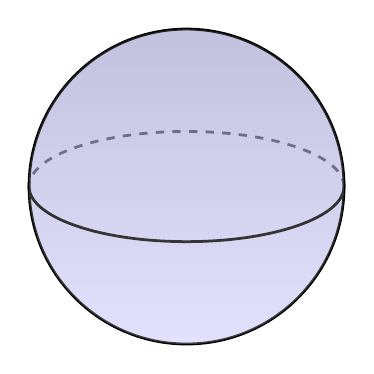
\begin{tikzpicture}[scale=2]
  \draw[line width=1, dashed] (1,0) arc (0:180:1 and 0.35);
  \draw[fill=blue!30!white!,opacity=0.5] (0,0) circle (1);
  \draw[line width=1] (1,0) arc (0:180:1 and -0.35);
  \draw[line width=1](0,0) circle (1);
  \shade[opacity=0.25] (0,0) circle (1);
\end{tikzpicture}


	\caption{La esfera $\S^{2}$ es una variedad topológica.}
\end{figure}

\begin{example}[Producto Finito de Variedades]\label{Ex: Variedad Topologica - Producto de Variedades}
	Si $M_1, \hdots, M_k$ son variedades topológicas de dimensiones $n_1,\hdots,n_k$ respectivamente, entonces $M = \Pi_{i=1}^k M_i$ es una variedad topológica de dimensión $\sum_{i=1}^k n_i$.

	En efecto, comencemos considerando el caso del producto de dos variedades. Sean $M_{1}^{n_1}$ y $M_{2}^{n_2}$ variedades topológicas. Como el producto arbitrario de espacios de Hausdorff es Hausdorff, tendremos que $M_1 \times M_2$ es Hausdorff. Además, como el producto numerable de espacios segundo numerables es segundo numerable $M_1 \times M_2$ es segundo numerable.
	Para cada punto $(x,y) \in M_1 \times M_2$ existirá un conjunto abierto $U \times V$ donde $U$ es el dominio de una carta $(U,\phi)$ en $M_1$ que contiene que a $x$ y $V$ es el dominio de una carta $(V,\psi)$ que contiene a $y$, por definición de cartas coordenadas $\phi: U \to \R^{n_1}$ y $\psi: V \to \R^{n_2}$ son homeomorfismo, por lo que podemos definir la función $F: U \times V \to \R^{n_1 + n_2}$ como:
	\[
		F(x,y) = (\phi(x),\psi(y)).
	\]

	Dado que $\phi$ y $\psi$ son homeomorfismo en particular serán funciones continuas, por lo que podemos garantizar que $F$ es continua y además es invertible, en particular, su inversa estará dada por $F^{-1}(a,b) = (\phi^{-1}(a),\psi^{-1}(b))$ y como las inversas de $\phi$  y $\psi$ también son continuas $F^{-1}$ es un mapa continuo. Así, $F$ es un homeomorfismo de $U \times V$ sobre $\R^{n_1 + n_2}$, como esto se cumple para cada punto $(x,y) \in M_1 \times M_2$ podemos concluir que el producto $M_1 \times M_2$ es una variedad topológica.

	El caso para el producto finito de variedades topológicas se sigue por inducción.
\end{example}

\begin{example}[$n-$Toro]\label{Ex: Variedad Topologica - Toro}
	El toro $n$-dimensional, que se denota por $\T^n$, y que se define como:
	\[
		\T^n = \underbrace{\S^1 \times \hdots \times \S^1}_{n-\text{veces}}.
	\]

	Esto se puede ver a partir de los ejemplos \ref{Ex: Variedad Topologica - Esfera} y \ref{Ex: Variedad Topologica - Producto de Variedades}, ya que son el producto finito de variedades topológicas.
\end{example}

\begin{figure}[h]
	\centering
	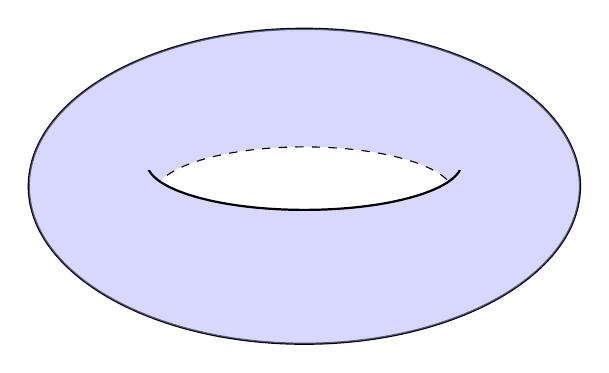
\begin{tikzpicture}[scale=2]
  % Elipse Principal
	\draw [thick] (0,0) ellipse  (1.75 and 1);
	\path[fill=blue!30!white,opacity=0.5] (0,0) ellipse  (1.75 and 1);

	%Arco inferior
	\begin{scope}
		\clip (0,0.15) ellipse (1 and 0.3);
		\fill[white] (0,-0.05) ellipse (0.95 and 0.3);
	\end{scope}

	% Arco superior
	\begin{scope}
		\clip (-1.25,0.03) rectangle (1.25,0.5);
		\draw[dashed] (0,-0.05) ellipse (0.95 and 0.3);
	\end{scope}

  % Centro
	\begin{scope}
		\clip (-1.25,0.1) rectangle (1.25,-0.5);
		\draw[thick] (0,0.15) ellipse (1 and 0.3);
	\end{scope}
\end{tikzpicture}

	\caption{El toro $\mathbb{T}^{2}$ es una variedad topológica.}
\end{figure}
